\documentclass{../../oss-apphys-exam}
\newcounter{last}

\begin{document}
\genheader

\gentitle{11}{UNIVERSAL GRAVITATION}

%\genmultidirections
%\gengravity

\raggedcolumns
\begin{multicols*}{2}
  \begin{questions}
    \question A \SI{70}{\kilo\gram} astronaut floats at a distance of
    \SI{10}{\metre} from a \SI{50000}{\kilo\gram} spacecraft. What is the force
    of attraction between the astronaut and spacecraft?
    \begin{choices}
      \choice\SI{2.4e-6}\newton
      \choice\SI{2.4e-5}\newton
      \choice Zero; there is no gravity in space.
      \choice\SI{2.4e5}\newton
      \choice\SI{2.4e6}\newton
    \end{choices}
    \vspace{.5in}
    
%    \question The Earth is at an average distance of \SI1{AU} from the Sun and
%    has an orbital period of \SI1{year}. Jupiter orbits the Sun at
%    approximately \SI5{AU}. About how long is the orbital period of Jupiter?
%    \begin{choices}
%      \choice\SI1{year}
%      \choice\SI2{years}
%      \choice\SI5{years}
%      \choice\SI{11}{years}
%      \choice\SI{125}{years}
%    \end{choices}
    
    \question A proposed ``space elevator'' can lift a \SI{1000}{\kilo\gram}
    payload to an orbit of \SI{150}{\kilo\metre} above the Earth's surface. The
    radius of the Earth is \SI{6.4e6}\metre, and the Earth's mass is
    \SI{6.e24}{\kilo\gram}. What is the gravitational potential energy of the
    payload when it reaches orbit?
    \begin{choices}
      \choice\SI{-1.0e3}\joule
      \choice\SI{-2.7e6}\joule
      \choice\SI{-6.1e10}\joule
      \choice\SI{-2.7e12}\joule
      \choice\SI{-1.0e15}\joule
    \end{choices}
    
%    \question A satellite orbits the Earth at a distance of
%    \SI{200}{\kilo\metre} in a circular path. If the mass of the Earth is
%    \SI{6.e24}{\kilo\gram} and the Earth's radius is \SI{6.4e6}\metre, what is
%    the satellite's speed?
%    \begin{choices}
%      \choice\SI{1.e3}{\metre\per\second}
%      \choice\SI{3.5e3}{\metre\per\second}
%      \choice\SI{7.8e3}{\metre\per\second}
%      \choice\SI{5e6}{\metre\per\second}
%      \choice\SI{6.1e7}{\metre\per\second}
%    \end{choices}
%    
%    \question Mars orbits the Sun at a distance of \SI{2.3e11}\metre. The
%    mass of the Sun is \SI{2.e30}{\kilo\gram}, and the mass of Mars is
%    \SI{6.4e23}{\kilo\gram}. Approximately what is the gravitational force that
%    the Sun exerts on Mars?
%    \begin{choices}
%      \choice\SI{1.6e20}{\newton}
%      \choice\SI{1.6e21}{\newton}
%      \choice\SI{3.7e21}{\newton}
%      \choice\SI{3.7e32}{\newton}
%      \choice\SI{3.7e42}{\newton}
%    \end{choices}

    \question The mass of a planet is $1/4$ that of Earth and its radius is
    half of Earth's radius. The acceleration due to gravity on this planet is
    most nearly
    \begin{choices}
      \choice\SI2{\metre\per\second\squared}
      \choice\SI4{\metre\per\second\squared}
      \choice\SI5{\metre\per\second\squared}
      \choice\SI{10}{\metre\per\second\squared}
      \choice\SI{20}{\metre\per\second\squared}
    \end{choices}
    
%    \question When climbing from sea level to the top of Mount Everest, a hiker
%    changes elevation by \SI{8848}\metre. By what percentage will the
%    gravitational field of the Earth change during the climb? (The Earth's
%    mass is \SI{6.e24}{\kilo\gram}, and its radius is \SI{6.4e6}\metre.)
%    \begin{choices}
%      \choice It will increase by approximately \SI{.3}\percent.
%      \choice It will decrease by approximately \SI{.3}\percent.
%      \choice It will increase by approximately \SI{12}\percent.
%      \choice It will decrease by approximately \SI{12}\percent.
%      \choice The gravitational field strength will not change.
%    \end{choices}
%    \vspace{.7in}

    \columnbreak
    \question Four planets, A through D, orbit the same star. The relative
    masses and distances from the star for each planet are shown in the table.
    For example, Planet A has twice the mass of Planet B, and Planet D has
    three times the orbital radius of Planet A. Which planet has the highest
    gravitational attraction to the star?
    \begin{center}
      \vspace{-.1in}
      \begin{tabular}{lll}
        \hline
        \textbf{Planet} & \textbf{Relative mass} & \textbf{Relative distance}\\
        \hline
        A\hspace{.4in}& $2m$     & $r$    \\ \hline
        B & $m$                  & $0.1r$\hspace{.25in} \\ \hline
        C & $0.5m$\hspace{.25in} & $2r$   \\ \hline
        D & $4m$                 & $3r$   \\ \hline
      \end{tabular}
    \end{center}
    \begin{choices}
      \choice Planet A
      \choice Planet B
      \choice Planet C
      \choice Planet D
      \choice All have the same gravitational attraction to the star.
    \end{choices}
    
    \question A satellite orbits the Earth at a distance that is four times the
    radius of the Earth. If the acceleration due to gravity near the surface of
    the Earth is $g$, the acceleration of the satellite is most nearly
    \begin{choices}
      \choice zero
      \choice $\dfrac g2$
      \choice $\dfrac g4$
      \choice $\dfrac g8$
      \choice $\dfrac g{16}$
    \end{choices}
  
%    \question A satellite orbits the Earth in an elliptical orbit, with point A
%    being close to the Earth and point B farther away. As the satellite moves
%    from point A to point B, which of the following is true of the angular
%    momentum and kinetic energy of the satellite?
%    \begin{center}
%      \vspace{-.1in}
%      \begin{tikzpicture}[scale=1.4]
%        \tikzstyle{balloon}=[ball color=gray];
%        \draw ellipse (2 and 1);
%        \fill( 2,0) circle(.05) node[right]{A};
%        \fill(-2,0) circle(.05) node[left]{B};
%        \shade[balloon] (.5,0) circle (.2);
%      \end{tikzpicture}
%    \end{center}
%  
%    \begin{tabular}{lll}
%      & \underline{Angular momentum} & \underline{Kinetic energy}\\
%      (A) & Increases & Remains constant \\
%      (B) & Remains constant & Increases \\
%      (C) & Decreases & Remains constant \\
%      (D) & Remains constant & Decreases \\
%      (E) & Remains constant & Remains constant
%    \end{tabular}
%    \vspace{.7in}
    
    \question Two planets of mass $M$ and $9M$ are in the same solar system. The
    radius of the planet of mass $M$ is $R$. In order for the acceleration due
    to gravity to be the same for each planet, the radius of the planet of mass
    $9M$ would have to be
    \begin{choices}
      \choice $\dfrac R2$
      \choice $R$
      \choice $2R$
      \choice $3R$
      \choice $9R$
    \end{choices}
    
%    \question A satellite is in a stable circular orbit around the Earth at a
%    radius $R$ and speed $\varv$. At what radius would the satellite travel in
%    a stable orbit with a speed $2\varv$?
%    \begin{choices}
%      \choice $\dfrac R4$
%      \choice $\dfrac R2$
%      \choice $R$
%      \choice $2R$
%      \choice $4R$
%    \end{choices}
%
%    \question Two planets, X and Y, orbit a star. Planet X orbits at a radius
%    $R$, and Planet Y orbits at a radius $3R$. Which of the following best
%    represents the relationship between the acceleration $a_X$ of Planet X and
%    the acceleration $a_Y$ of Planet Y?
%    \begin{center}
%      \begin{tikzpicture}[scale=.7]
%        \tikzstyle{balloon}=[ball color=gray];
%        \shade[balloon] circle(.25);
%        \draw[dashed] circle(1);
%        \draw[dashed] circle(3);
%        \draw(0,0)--(1,0) node[right]{X} node[midway,above]{$R$};
%        \draw[fill=black](1,0) circle(.05);
%        \begin{scope}[rotate=230]
%          \draw(0,0)--(3,0) node[left]{Y} node[pos=.7,right]{$3R$};
%          \draw[fill=black](3,0) circle(.05);
%        \end{scope}
%      \end{tikzpicture}
%    \end{center}
%    \begin{choices}
%      \choice $a_X = 9a_Y$
%      \choice $9a_X = a_Y$
%      \choice $a_X = 3a_Y$
%      \choice $3a_X = a_Y$
%      \choice $a_X = a_Y$
%    \end{choices}
%
%    \question A planet orbits at a radius $R$ around a star of mass $M$. The
%    period of orbit of the planet is
%    \begin{choices}
%      \choice $\sqrt{\dfrac{4\pi^2R^2}{GM}}$
%      \choice $\dfrac{4\pi^2R^3}{GM}$
%      \choice $\sqrt{\dfrac{4\pi^2R^3}{GM}}$
%      \choice $\sqrt{\dfrac{4\pi^2R}{GM}}$
%      \choice $\dfrac{GM}{4\pi^2R}$
%    \end{choices}
%
%    \question A moon orbits a large planet in an elliptical orbit, with its
%    closest approach at a distance $a$, and its farthest distance $b$. The
%    speed of the moon at point b is $\varv$. The speed at point $a$ is
%    \begin{choices}
%      \choice $\dfrac{a\varv}b$
%      \choice $\dfrac{b\varv}a$
%      \choice $\dfrac{(a+b)\varv}b$
%      \choice $\dfrac{(b-a)\varv}b$
%      \choice $\dfrac{2b\varv}a$
%    \end{choices}
%
%    \question A satellite orbits the Earth in an elliptical orbit. Which of the
%    following statements is true?
%    \begin{choices}
%      \choice The angular velocity of the satellite increases as it travels
%      farther from the Earth.
%      \choice The acceleration of the satellite increases as it travels closer
%      to the Earth.
%      \choice The angular momentum of the satellite increases as it travels
%      closer to the Earth.
%      \choice The potential energy of the satellite is equal to its kinetic
%      energy at all points in the orbit.
%      \choice The speed of the satellite must remain constant for it to remain
%      in orbit around the Earth.
%    \end{choices}
%    \vspace{.7in}
%    \columnbreak

    \uplevel{
      \textbf{Questions \ref{moon1}--\ref{moon2}}
      
      Two moons of mass $m$ and $2m$ orbit a planet of mass $M$ at the same
      radius $R$ and speed $\varv$ toward each other, as shown. The moons
      collide and stick together without destroying either moon.
      \begin{center}
        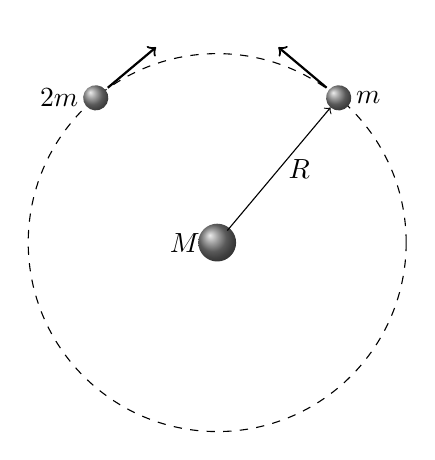
\begin{tikzpicture}[scale=.8]
          \tikzstyle{balloon}=[ball color=gray];
          \shade[balloon] circle(.3) node[left]{$M\;$};
          \draw[dashed] circle(3);
          \begin{scope}[rotate=50]
            \draw[->](0.25,0)--(2.8,0) node[midway,right]{$R$};
            \shade[balloon] (3,0) circle (.2) node[right]{$\;m$};
            \draw[thick,->](3,0.25)--(3,1.25) node[above]{$\varv$};
          \end{scope}
          \begin{scope}[rotate=130]
            \shade[balloon] (3,0) circle (.2) node[left]{$2m\;$};
            \draw[thick,->](3,-0.25)--(3,-1.25) node[above]{$\varv$};
          \end{scope}
        \end{tikzpicture}
      \end{center}
    }
    
    \question The total momentum of the moons after the collision is
    \begin{choices}
      \choice $m\varv$
      \choice $2m\varv$
      \choice $3m\varv$
      \choice $6m\varv$
      \choice zero
    \end{choices}
    \label{moon1}
    
    \question The velocity of the two masses after the collision above is
    \label{moon2}
    \begin{choices}
      \choice $\varv$ counterclockwise
      \choice $\varv/2$ counterclockwise
      \choice $\varv/2$ clockwise
      \choice $\varv/3$ counterclockwise
      \choice $\varv/3$ clockwise
    \end{choices}
    \vspace{.7in}
    
%    \question A satellite of mass $m$ travels in an elliptical orbit around a
%    planet of mass $M$. The satellite has a speed $\varv$ when it is closest to
%    the planet at a distance $r$. Work is done by the engines of the satellite
%    to change its orbit to a circular orbit when it is at this distance $r$.
%    Which of the following statements is true of the transition from an
%    elliptical orbit to a circular orbit?
%    \begin{choices}
%      \choice The work done by the satellite engines to change the orbit is
%      equal to the change in kinetic energy of the satellite.
%      \choice The work done by the satellite engines to change the orbit is
%      equal to the change in potential energy of the satellite.
%      \choice The work done by the satellite engines to change the orbit is
%      equal to the change in angular momentum of the satellite.
%      \choice The work done by the satellite engines to change the orbit is
%      equal to the change in speed of the satellite.
%      \choice The work done by the satellite engines to change the orbit is
%      equal to the change in orbital radius of the satellite.
%    \end{choices}
%    \vspace{.7in}
%    
%    \question A satellite of mass $m$ orbits the Earth with a potential energy
%    $U$ and a kinetic energy $K$. Which of the following statements would have
%    to be true for the satellite to escape the Earth's gravity completely?
%    \begin{choices}
%      \choice The kinetic energy of the satellite would have to be equal to the
%      potential energy between the Earth and the satellite.
%      \choice The potential energy between the Earth and the satellite would
%      have to be greater than the kinetic energy of the satellite.
%      \choice The total energy of the satellite would have to be greater than
%      the kinetic energy of the satellite.
%      \choice The kinetic energy of the satellite would have to be greater than
%      the potential energy of the satellite.
%      \choice The total energy of the satellite would have to be equal to the
%      potential energy of the satellite.
    %    \end{choices}
  \end{questions}
  \setcounter{last}{\value{question}}
\end{multicols*}
\newpage

\genfreetitle{11}{UNIVERSAL GRAVITATION}{3}
%\genfreedirections

%  % TAKEN FROM THE 2007 AP PHYSICS C MECHANICS EXAM FREE-RESPONSE QUESTION 2
%  \question In March 1999 the Mars Global Surveyor (GS) entered its final orbit
%  about Mars, sending data back to Earth. Assume a circular orbit with a period
%  of $\SI{1.18e2}{minutes}=\SI{7.08e3}\second$ and orbital speed of
%  \SI{3.40e3}{\metre\per\second}. The mass of the GS is \SI{930}{\kilo\gram}
%  and the radius of Mars is \SI{3.43e6}\metre.
%  \begin{parts}
%    \part Calculate the radius of the GS orbit.
%    \part Calculate the mass of Mars.
%    \part Calculate the total mechanical energy of the GS in this orbit.
%    \part If the GS was to be placed in a lower circular orbit (closer to the
%    surface of Mars), would the new orbital period of the GS be greater than or
%    less than the given period? Justify your answer.
%
%    \vspace{.15in}
%    \underline{\hspace{.3in}} Greater than\hspace{1in}
%    \underline{\hspace{.3in}} Less than
%
%    \part In fact, the orbit the GS entered was slightly elliptical with its
%    closest approach to Mars at \SI{3.71e5}{\metre} above the surface and its
%    furthest distance at \SI{4.36e5}{\metre} above the surface. If the speed of
%    the GS at closest approach is \SI{3.40e3}{\metre\per\second}, calculate the
%    speed at the furthest point of the orbit.
%  \end{parts}
%  \newpage
%  
%  % TAKEN FROM THE 2005 AP PHYSICS C MECHANICS EXAM FREE-RESPONSE QUESTION 2
%  \question A student is given the set of orbital data for some of the moons of
%  Saturn shown below and is asked to use the data to determine the mass $M_S$
%  of Saturn. Assume the orbits of these moons are circular.
%  \begin{center}
%    \def\arraystretch{1.5}
%    \begin{tabular}{|c|c|p{1in}|p{1in}|}
%      \hline
%      Orbital Period, $T$ &  Orbital Radius, $R$ & & \\
%      (seconds)           &  (meters)            & & \\
%      \hline
%      \num{8.14e4} & \num{1.85e8} & & \\ \hline
%      \num{1.18e5} & \num{2.38e8} & & \\ \hline
%      \num{1.63e5} & \num{2.95e8} & & \\ \hline
%      \num{2.37e5} & \num{3.77e8} & & \\ \hline
%    \end{tabular}
%  \end{center}
%  \def\arraystretch{1}
%  \begin{parts}
%    \part Write an algebraic expression for the gravitational force between
%    Saturn and one of its moons.
%    \label{algebraic}
%    
%    \part Use your expression from part (\ref{algebraic}) and the assumption of
%    circular orbits to derive an equation for the orbital period $T$ of a moon
%    as a function of its orbital radius $R$.
%    
%    \part Which quantities should be graphed to yield a straight line whose
%    slope could be used to determine Saturn's mass?
%
%    \part Complete the data table by calculating the two quantities to be
%    graphed. Label the top of each column, including units.
%
%    \part Plot the graph on the axes below. Label the axes with the variables
%    used and appropriate numbers to indicate the scale.
%    \cpic{.8}{graph-paper}
%    \part Using the graph, calculate a value for the mass of Saturn.
%  \end{parts}
%  \newpage

\begin{center}
  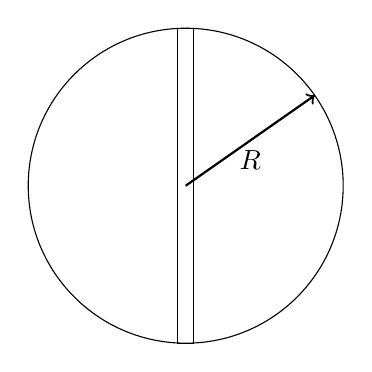
\begin{tikzpicture}
    \draw circle(2);
    \draw(-0.1,2) rectangle(0.1,-2);
    \draw[->,thick,rotate=35](0,0)--(2,0) node[midway,below]{$R$};
  \end{tikzpicture}
\end{center}
\begin{questions}
  \setcounter{question}{\value{last}}
  
  \question A planet of mass $M$, radius $R$, and uniform density has a small
  tunnel drilled through the center of the planet, as shown above. When the
  mass is inside the tunnel, it experiences a force of $F=(GmM/R^3)r$, whereas
  when the mass is outside of the planet, it experiences a gravitational force
  of $F=GmM/r^2$.
  \begin{parts}
    \part Setting the potential energy of the mass to be zero at the planet's
    center, calculate the mass's potential energy as a function of distance from
    the center of the planet $U(r)$, for values $r<R$. Sketch this potential
    function.
    \vspace{\stretch1}
    
    \part If the mass is dropped from $R$ from the center of the planet, how
    long will it take until it returns to its original position?
    \vspace{\stretch1}
    
    \part If the mass is dropped from $R/2$ from the center of the planet, will
    it require more, or less, or the same amount of time to return to its
    original position compared to if it was dropped from $R$?
    \vspace{\stretch1}
    
    \part If the mass is dropped from $2R$ from the center of the planet, will
    it require more, or less, or the same amount of time to return to its
    original position compared to if it was dropped from $R$?
    \vspace{\stretch1}
  \end{parts}
  \newpage

  \question Two stars of unequal mass orbit each other about their common
  center of mass as shown. The star of mass $M_1$ orbits in a circle of radius
  $r$, and the star of mass $M_2$ orbits in a circle of radius $2r$.
  \begin{center}
    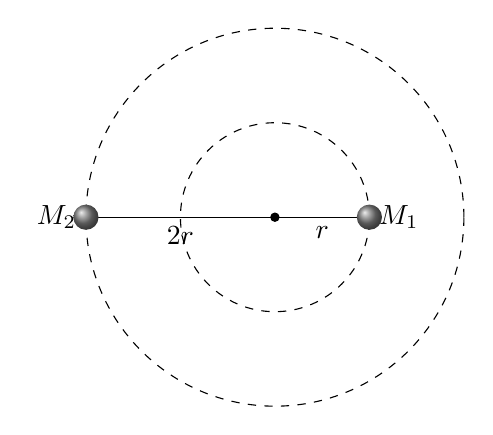
\begin{tikzpicture}[scale=.8]
      \fill circle(.075);
      \draw[dashed] circle(3);
      \draw[dashed] circle(1.5);
      \draw[->](0,0)--(1.5,0) node[midway,below]{$r$};
      \shade[ball color=gray] (1.5,0) circle(.2) node[right]{$M_1$};
      \draw[->](0,0)--(-3,0) node[midway,below]{$2r$};
      \shade[ball color=gray] (-3,0) circle(.2) node[left]{$M_2$};
    \end{tikzpicture}
  \end{center}
  \begin{parts}
    \part Determine the ratio of masses $M_1/M_2$.
    \vspace{\stretch1}
    
    \part Determine the ratio of the acceleration $a_1$ of $M_1$ to the
    acceleration $a_2$ of $M_2$.
    \vspace{\stretch1}
    
    \part Determine the ratio of the period $T_1$ of $M_1$ to the period $T_2$
    of $M_2$.
    \vspace{\stretch1}
  \end{parts}
  \newpage

  % TAKEN FROM THE 2001 AP PHYSICS C FREE-RESPONSE QUESTION MECH.2
  \question An explorer plans a mission to place a satellite into a circular
  orbit around the planet Jupiter, which has mass $M_J=\SI{1.90e27}{\kilo\gram}$
  and radius $R_J=\SI{7.14e7}\metre$.
  \begin{parts}
    \part If the radius of the planned orbit is $R$, use Newton's laws to show
    each of the following.
    \begin{subparts}
      \subpart The orbital speed of the planned satellite is given by
      $\varv=\sqrt{\dfrac{GM_J}R}$.
      \vspace{\stretch1}
      
      \subpart The period of the orbit is given by
      $T=\sqrt{\dfrac{4\pi^2R^3}{GM_J}}$.
      \vspace{\stretch1}
    \end{subparts}
    
    \part The explorer wants the satellite's orbit to be synchronized with
    Jupiter's rotation. This requires an equatorial orbit whose period equals
    Jupiter's rotation period of 9 hr 51 min = \SI{3.55e4}\second. Determine
    the required orbital radius in meters.
    \vspace{\stretch1}
    \newpage
    
    \part Suppose that the injection of the satellite into orbit is less than
    perfect. For an injection velocity that differs from the desired value in
    each of the following ways, sketch the resulting orbit on the figure. ($J$
    is the center of Jupiter, the dashed circle is the desired orbit, and $P$
    is the injection point.) Also, describe the resulting orbit qualitatively
    but specifically.    
    \begin{subparts}
      \subpart When the satellite is at the desired altitude over the equator,
      its velocity vector has the correct direction, but the speed is slightly
      faster than the correct speed for a circular orbit of that radius.
      \uplevel{
        \centering
        \vspace{.4in}
        \begin{tikzpicture}[scale=.8]
          \draw[thick,dashed] circle(2);
          \fill circle(.08) node[below]{$J$};
          \fill(0,2) circle(.08) node[above]{$P$};
        \end{tikzpicture}
        \vspace{.4in}
      }
      \subpart When the satellite is at the desired altitude over the equator,
      its velocity vector has the correct direction, but the speed is slightly
      slower than the correct speed for a circular orbit of that radius.
      \uplevel{
        \centering
        \vspace{.4in}
        \begin{tikzpicture}[scale=.8]
          \draw[thick,dashed] circle(2);
          \fill circle(.08) node[below]{$J$};
          \fill(0,2) circle(.08) node[above]{$P$};
        \end{tikzpicture}
        \vspace{.4in}
      }
    \end{subparts}
  \end{parts}
  
  % THIS QUESTION CAME FROM THE TIPLER TEXTBOOK. IT CAN BE RE-USED FOR OTHER
  % COURSES IN THE FUTURE.
%  \question Two point particles of mass $m$ are on the $y$ axis at $y=a$ and
%  $y=-a$, as shown in the figure below.
%  \begin{center}
%    \begin{tikzpicture}[scale=.7]
%      \tikzstyle{balloon1}=[ball color=green!50!gray];
%      \tikzstyle{balloon2}=[ball color=red!50];
%      \draw[->](-2,0)--(6,0) node[right]{$x$};
%      \draw[->](0,-3)--(0,3) node[above]{$y$};
%      \draw[<->](-1,0)--(-1,2) node[midway,left]{$a$};
%      \draw[<->](-1,0)--(-1,-2)node[midway,left]{$a$};
%      \draw(0,2)--(-1.2,2);
%      \draw(0,-2)--(-1.2,-2);
%      \shade[balloon1] (0,2) circle (.55) node[white]{$m$};
%      \shade[balloon1] (0,-2)circle (.55) node[white]{$m$};
%      \shade[balloon2] (4,0) circle (.45) node[white]{$m_0$};
%    \end{tikzpicture}
%  \end{center}
%  \begin{parts}
%    \part Derive the expression for the gravitational force exerted by these two
%    particles on a third particle of mass $m_0$ located on the $x$ axis at a
%    distance $x$ away from the origin.
%    
%    \part What is the gravitational field $\vec g$ on the $x$-axis due to the
%    two particles?
%    
%    \part Show that $g_x$ (the $x$ component of $\vec g$) due to the two
%    particles on the $y$ axis is approximately $-\dfrac{2Gm}{x^2}$ when $x$ is
%    much greater than $a$.
%    
%    \part Show that the maximum value of $|g_x|$ occurs at the point
%    $x=\dfrac{\pm a}{\sqrt2}$.
%  \end{parts}
%  \newpage

  
%\item\textbf{THIS IS A CHALLENGE PROBLEM THAT IS MORE DIFFICULT THAN AP EXAMS:}
%  Spacecraft that study the Sun are often placed at the ``L1 Lagrange Point'',
%  located sunward of Earth on the Sun--Earth line. L1 is the point where Earth's
%  and Sun's gravity together produce an orbital period of one year, so that a
%  spacecraft at L1 stays fixed relative to Earth as both planet and spacecraft
%  orbit the Sun. This placement ensures an uninterrupted view of the sun,
%  without being periodically eclipsed by Earth as would occur in Earth orbit.
%  Find L1's location relative to Earth. (Hint: This problem calls for numerical
%  methods for solving high-order polynomial equation.)

\end{questions}
\end{document}
